\documentclass[a4paper,12pt,twoside]{article}%twoside
\usepackage[utf8]{inputenc}
\usepackage[dutch]{babel}
\usepackage{fancyhdr, amsmath, color, graphicx, enumitem, tabularx, hyperref, longtable, multirow, placeins, apacite, subcaption,marvosym,multicol}
\usepackage[framemethod=tikz]{mdframed}
 \usetikzlibrary{positioning}
  \usepackage[margin=2.5cm,headheight=68pt]{geometry}
 %\usepackage[total={16cm, 22cm}]{geometry}
 
\pagestyle{fancy}
\fancyhf{}
\fancyhead[LE,RO]{}%'E': even page, 'O': odd page
\fancyhead[RE,LO]{Correctiesleutels bij oefeningen op flux, inductiespanning en inductiestroom}
\fancyfoot[C]{K. Truyaert}
\fancyfoot[LE,RO]{5TW Toegepaste fysica}
\fancyfoot[LO,RE]{\thepage}
%\renewcommand{\labelitemi}{$\circ$}
 
\definecolor{CVO}{RGB}{232, 0, 97}
\setlength\parindent{0pt}

 %Strikeout and highlight text
  \usepackage{soul}
  \usepackage{tikz} % only to get \foreach
  
  %\definecolor{yellow}{RGB}{255,255,0}
  \sethlcolor{yellow}
 
 \begin{document}
\underline{Oefening 6}\newline	Een rechte geleider van 0,500~m lengte wordt met een snelheid van 2,00~m/s doorheen een homogeen magnetisch veld bewogen loodrecht op de veldlijnen. Hierdoor ontstaat tussen de uiteinden van de geleider een inductiespanning van 3,00~V. 
Bereken de grootte van de magnetische veldsterkte van dit magnetisch veld.\\

\underline{Gegeven:}\newline
l = 0,500~m\\
v = 2,00~m/s\\
U$_i$ = 3,00~V\\
\\
\underline{Gevraagd:}\\
B\\ \\
\underline{Oplossing:}\\
In deze vraag beweeg je een rechte geleider loodrecht op een magnetisch veld. Deze situatie gebeurt in onderstaande afbeelding, waar de staaf van links naar rechts  door het magnetisch veld beweegt:
\begin{figure}[h]
	\centering
	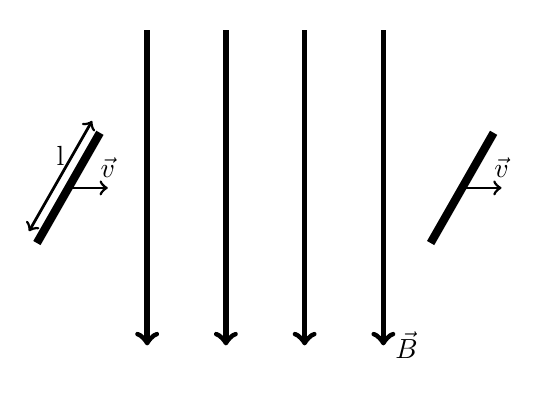
\begin{tikzpicture}
		\draw[->,line width = 2pt] (4,2)--(4,-2) node[right]{$\vec{B}$};
		\draw[->,line width = 2pt] (1,2)--(1,-2);
		\draw[->,line width = 2pt] (2,2)--(2,-2);
		\draw[->,line width = 2pt] (3,2)--(3,-2);
		\draw[-,line width = 3pt] (-0.4,-0.7)--(0.4,0.7);
		\draw[<->,line width = 1pt] (-0.5,-0.55)--(0.3,0.85) node[midway,above]{l};
		\draw[->,line width = 1pt] (0,-0)--(0.5,0) node[above] {$\vec{v}$};
		\draw[-,line width = 3pt] (4.6,-0.7)--(5.4,0.7);
		\draw[->,line width = 1pt] (5,-0)--++(0.5,0) node[above] {$\vec{v}$};
	\end{tikzpicture}
\end{figure}

De grootte van het magnetisch veld kan je via het inductieverschijnsel in een rechte, bewegende geleider vinden. Hiervoor gebruik je de vergelijking:\[\left|U_i\right|= NBlv.\]
Deze vergelijking omvormen naar $B$ levert de volgende vergelijking op:
\[B = \frac{\left|U_i\right|}{Nlv}.\]
Invullen van alle gekende factoren (N=1), levert een magnetische veldsterkte van 3,00~T op.


\newpage






\underline{Oefening 7}\newline	We trekken een rechte draad van 50,0~cm lang, die deel uitmaakt van een stroomkring met totale weerstand 0,0100~$\Omega$, met een snelheid van 5,00~m/s doorheen een homogeen magnetisch veld met veldsterkte 0,700~T. Bewegingsrichting, draad en magnetische veldlijnen staan loodrecht op elkaar. 
Bereken tijdens deze beweging :
\begin{enumerate}
	\item de inductiespanning
	\item	de inductiestroom
	\item	de kracht die de draad vanwege het magnetisch veld ondervindt
\end{enumerate} 

\underline{Gegeven:}\newline
l = 0,500~m\\
v = 5,00~m/s\\
R = 0,0100~$\Omega$\\
B = 0.700~T
\\ \\
\underline{Gevraagd:}
\begin{enumerate}
	\item U$_i$
	\item I$_i$
	\item F
\end{enumerate} 
\underline{Oplossing:}\\
\begin{enumerate}
	\item In deze vraag beweeg je een rechte geleider loodrecht op een magnetisch veld. Deze geleider is een halve meter lang en is onderdeel van een grotere stroomkring. De inductiespanning bepaal je opnieuw via de vergelijking van het inductieverschijnsel in een rechte, bewegende geleider vinden:\[\left|U_i\right|= NBlv.\]
	In dit geval levert dat dus een inductiespanning van $\left|U_i\right| = 1,75~V$ op.
	\item Deze spanning zal dus door de stroomkring lopen. De weerstand van die stroomkring is gekend. Via de wet van Ohm kan je dus de waarde van de inductiestroom gaan bepalen:
	\[I_i = \frac{U_i}{R} = 175~A.\]
	\item De kracht op de bewegende geleider bepaal je via de Lorentzkracht:\[F = BIl = 61,3~N.\]
\end{enumerate}
\newpage


\underline{Oefening 8}\newline	Een magnetisch veld met lengte 240~cm verdwijnt loodrecht in het vlak van dit blad. Een blokje met lengte l beweegt rechtlijnig naar rechts door dit veld met snelheid v. De magnetische flux door het blokje wordt gedurende deze beweging voorgesteld als functie van de tijd in de rechtergrafiek.
\begin{enumerate}
	\item Bereken de lengte van het blokje.
	\item Met welke snelheid beweegt het blokje?
\end{enumerate} 

\underline{Gegeven:}\newline
d = 2,40~m\\

\underline{Gevraagd:}
\begin{enumerate}
	\item l
	\item v
\end{enumerate} 
\underline{Oplossing:}\\
In deze vraag beweeg je een rechthoekig blokje loodrecht op een magnetisch veld. Dit magnetisch veld is uitgespannen over een lengte $d$. Deze geleider beweegt zich in het magnetisch veld tussen $t=2~s$ en  $t=4~s$. Daarna is de maximale flux bereikt en blijft deze behouden tot $t= 10~s$. De flux wordt daarna terug kleiner, aangezien de rechthoekige geleider zich in een tijdspanne van 2 seconden uit het magnetisch veld verwijdert. \\
De geleider doet er dus 2 seconden over om zijn volledige lengte af te leggen, aangezien de maximale flux na 2 seconden bereikt wordt. We weten dus dat, aglemeen, $\Delta s = v\Delta t$, ofwel dat in dit geval geldt dat $l = v\cdot 2~s$.\\
Nu het blokje volledig in het magnetisch veld hangt, blijft de flux tussen $t=4~s$ en $t=10~s$ constant. In die tijdspanne legt het blokje opnieuw een afstand $\Delta s$, nu gelijk aan $v\cdot 6~s$ af, die ditmaal gelijk is aan 2,40~m-l, zoals te zien is in onderstaande figuur:
\begin{figure}[!h]
	\centering
	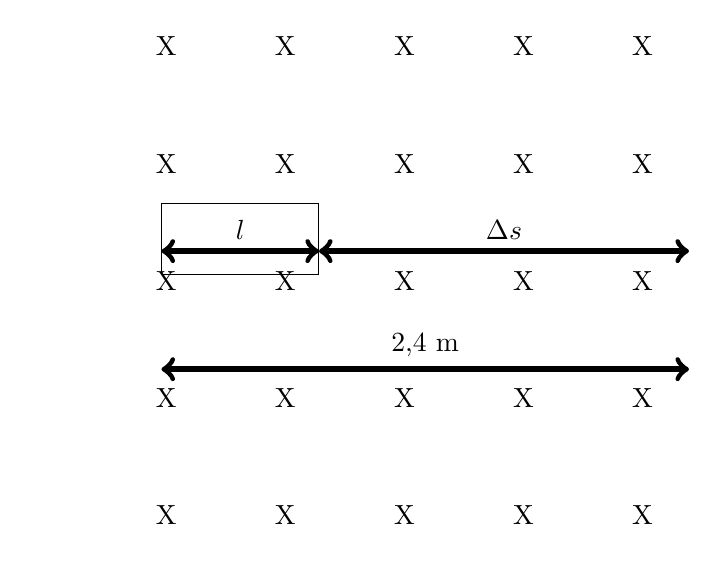
\begin{tikzpicture}
	\node[white] (n00) {X};
	\foreach \x [remember=\x as \lastx (initially 0)] in {0,...,4}{
		\node[right =of n\lastx0] (n\x0) {X};
		\foreach \y [remember=\y as \lasty (initially 0)] in {1,...,4}{
			\node[below =of n\x\lasty] (n\x\y) {X};
		}
	}
	\draw(1.45,-2.9) rectangle (3.45,-2);	
	\draw[<->, line width = 2pt](1.45,-4.1) --++ (6.7,0) node[midway,above]{2,4~m};		
	\draw[<->, line width = 2pt](3.45,-2.6) --++ (4.7,0) node[midway,above]{$\Delta s$};		
	\draw[<->, line width = 2pt](1.45,-2.6) --++ (2,0) node[midway,above]{$l$};		
	\end{tikzpicture}
\end{figure}
We weten dus dat enerzijds $l = 2~s\cdot v$ en anderzijds dat $2,40~m=l+6~s\cdot v$. Na substitutie vind je dat $v = 0,3~m/s$ en dat $l=0,60~m$.
\newpage


\underline{Oefening 9}
Een cirkelvormige spoel bevat 20 windingen van 25,0~cm diameter en staat loodrecht op een homogeen magnetisch veld met grootte 0,0800~T. De spoel wordt in 5,00~ms een kwartslag om zijn middellijn gedraaid.


\underline{Gegeven:}\newline
N = 20\newline
d = 0,250~m $\rightarrow$ r = 0,125~m\\
B = 0,0800~T\\
$\Delta t$ = 5,00~ms = 0,00500~s

\underline{Gevraagd:}
$U_i$ \\
\underline{Oplossing:}\\
Je weet via de algemene inductiewet dat de grootte van de inductiespanning als volgt bepaald wordt:
\(\left|U_i\right|=N\frac{\Delta\Phi}{\Delta t}.\)
Hiervan is reeds alles gekend, behalve het verschil in flux. Aangezien de spoel een kwartslag draait, wijzigt de flux hier via een wijziging in de hoek $\alpha$.\newline
$\Phi_1 = BA\cos(0)=0,0800~T\cdot\pi 0,125^2~m^2\cdot 1= 0,00393~Wb$\newline
$\Phi_2 = BA\cos(90) = 0~Wb$\\
$\Rightarrow \Delta\Phi = -0,00393~Wb$
De grootte van de inductiespanning wordt dus:
\(\left|U_i\right|=N\frac{\Delta\Phi}{\Delta t}=20\cdot\frac{0,00393~Wb}{0,00500~s}=15,7~V.\)

De gemiddelde inductiespanning die doorheen de spoel vloeit is 15,7 Volt. 


\newpage



\underline{Oefening 11}\\
In een rechthoekig draadraam van 50,0 bij 10,0 cm is een lampje met een weerstand van 20,0 $\Omega$ opgenomen. Het draadraam wordt met een constante snelheid van 0,300 m/s in een homogeen magneetveld met een veldsterkte van 0,220 T geduwd.
\begin{figure}[!h]
	\centering
	\scalebox{0.25}{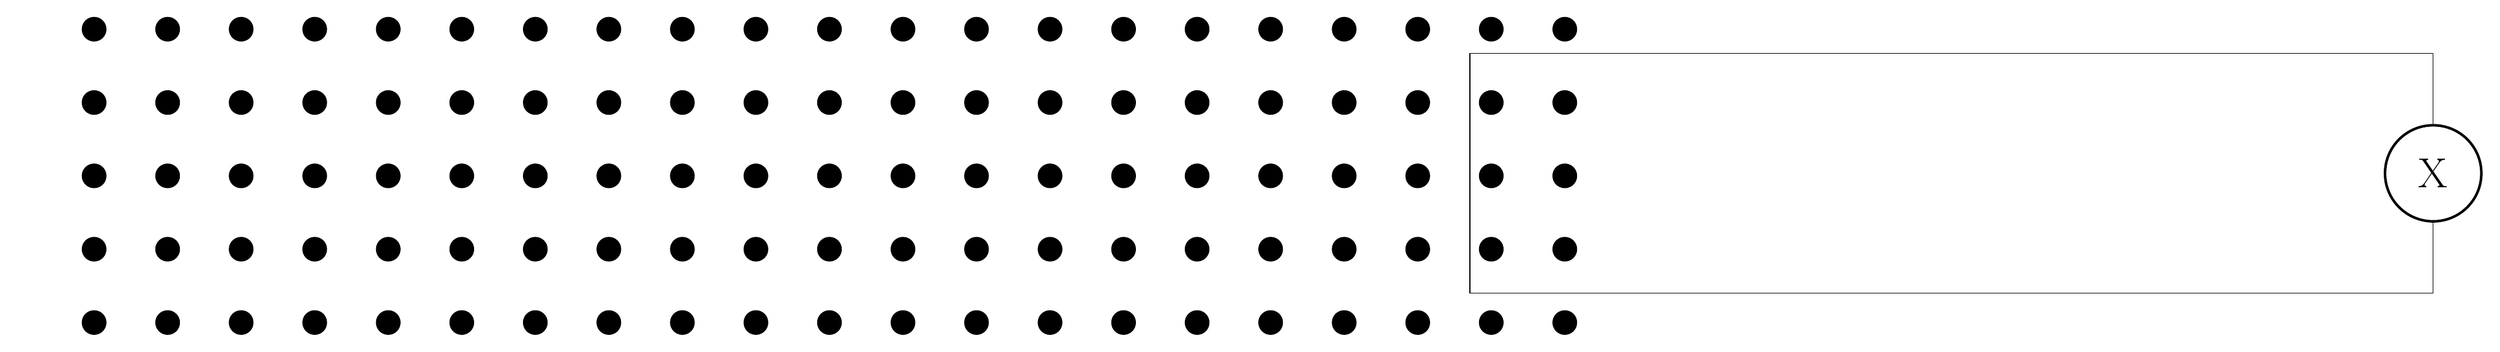
\begin{tikzpicture}
	\node[white] (c00) {$\cdot$};
	\foreach \x [remember=\x as \lastx (initially 0)] in {0,...,20}{
		\node[right =of c\lastx0,shape=circle,fill=black] (c\x0) {$\cdot$};
		\foreach \y [remember=\y as \lasty (initially 0)] in {1,...,4}{
			\node[below =of c\x\lasty,shape=circle,fill=black] (c\x\y) {$\cdot$};
		}
	}
	\draw(30,-5.5) rectangle (50,-0.5);	
	\draw[fill=white,line width=1.5pt] (50,-3) circle (1cm) node{\Huge X};
	\end{tikzpicture}}
\end{figure}
\begin{enumerate}
	\item[a)] Bereken hoeveel de flux door het draadraam per seconde toeneemt. 
	\item[b)] Bereken de inductiespanning die hierdoor in het draadraam wordt opgewekt. 
	\item[c)] Bereken de stroomsterkte in het draadraam en geef in de afbeelding aan in welke zin deze stroom loopt. 
	\item[d)] Bereken de grootte en richting van de Lorentzkracht die op het draadraam werkt. 
	\item[e)] Laat met een berekening zien dat het bij het duwen geleverde vermogen gelijk is aan het door het lampje verbruikte vermogen.
\end{enumerate}

\underline{Oplossing:}\\
\begin{enumerate}
	\item[a)] Een rechte bewegende geleider beweegt in een magnetisch veld. Hierdoor kunnen we zeggen dat de fluxverandering bepaald zal worden via: $\Delta\Phi = B~l~\Delta x$. De snelheid van het raam is gekend, dus er is geweten hoeveel afstand er per seconde afgelegd wordt. Hier is de fluxverandering: $\Delta\Phi = 0,220~T\cdot0,100~m\cdot0,300~m=0,00660~Wb$.
	\item[b)] Een rechte bewegende geleider beweegt in een magnetisch veld. Hierdoor kunnen we zeggen dat de inductiespanning bepaald zal worden via: $\Delta\Phi = B~l~v$. De snelheid van het raam is gekend, dus er is geweten hoeveel afstand er per seconde afgelegd wordt. Hier is de inductiespanning: $\Delta\Phi = 0,220~T\cdot0,100~m\cdot0,300~m/s=0,00660~V$
	\item[c)] In een gesloten kring wordt ook een stroom geïnduceerd wanneer een inductiespanning ontstaat. In deze kring is er een weerstand van 20,0~$\Omega$. Via de wet van Ohm vind je dus dat er een inductiestroom van $0,000330~A$, ofwel 330~$\mu$A in de kring vloeit. De stroom vloeit zo zodat het geïnduceerde magnetisch veld de fluxverandering tegenwerkt. Hier ontstaat er een fluxstijging, dus het geïnduceerde magnetisch veld zal tegengesteld zijn aan dat dat aangelegd is. Hierdoor vloeit de stroom in wijzerin op de figuur. 
	\item[d)] De Lorentzkracht op het raam werkt op het linkerstuk draad. Het magnetisch veld komt uit het blad, de stroom loopt verticaal op je blad naar boven. Via de linkerhandregel vind je dat de Lorentzkracht naar rechts georiënteerd is. De vergelijking voor de Lorentzkracht is F=BIL, wat in dit geval dus $7,26~\mu$N is.
	\item[e)] \underline{Vermogen van het duwen:}\newline
				P$_\text{duwen}$ = F$\cdot$v = 7,26~N$\cdot$0,300~m/s=2,18~$\mu$W\newline \underline{Vermogen van het lampje:}\newline
				P$_\text{lampje}$ = $U_i\cdot I_i$ = 0,00660~V$\cdot$0,00330~A=2,18~$\mu$W
\end{enumerate}



 \end{document}
